%
%   This file is part of the APS files in the REVTeX 4 distribution.
%   Version 4.0 of REVTeX, August 2001
%
%   Copyright (c) 2001 The American Physical Society.
%
%   See the REVTeX 4 README file for restrictions and more information.
%
% TeX'ing this file requires that you have AMS-LaTeX 2.0 installed
% as well as the rest of the prerequisites for REVTeX 4.0
%
% See the REVTeX 4 README file
% It also requires running BibTeX. The commands are as follows:
%
%  1)  latex apssamp.tex
%  2)  bibtex apssamp
%  3)  latex apssamp.tex
%  4)  latex apssamp.tex
%
%\documentclass[prb,aps,nobibnotes,twocolumn,doublespace,twocolumngrid,superbib]{revtex4}
%%\documentclass[twocolumn,showpacs,preprintnumbers,amsmath,amssymb]{revtex4}
%\documentclass[preprint,showpacs,preprintnumbers,amsmath,amssymb]{revtex4}

% Some other (several out of many) possibilities
%\documentclass[preprint,aps]{revtex4}
%\documentclass[preprint,aps,draft]{revtex4}
%\documentclass[prb]{revtex4}% Physical Review B

%%\usepackage{amsmath}
%%\usepackage{amssymb}
%%\usepackage{graphicx}% Include figure files
%%\usepackage{dcolumn}% Align table columns on decimal point
%%\usepackage{bm}% bold math


\documentclass[prl,aps,letterpaper,twocolumn,showpacs,twocolumngrid,superbib]{revtex4}

\usepackage{graphicx}
\usepackage{amsfonts}
\usepackage{amsmath}
\usepackage{bm}
\usepackage{alltt}
\usepackage{fancyhdr}

\pagestyle{fancy}

\def\Tr{{\rm Tr}}
\def\F{\mathcal{F}}
\def\D{\mathcal{D}}
\def\X{\mathcal{X}}
\def\E{\mathcal{E}}

%\nofiles

\begin{document}


\title{The Perturbed Projector for Higher Order Response in ${\cal O}(N)$} 

\author{Val\'ery Weber}
\email{valery.weber@unifr.ch}
\affiliation{Department of Chemistry, University of Fribourg, 1700 Fribourg, Switzerland.}
\author{Anders M. N. Niklasson}
\author{Matt Challacombe}
\affiliation{Los Alamos National Laboratory, Theoretical Division, Los Alamos 87545, New Mexico, USA.}

\date{\today}

\begin{abstract}
Perturbed projection  for linear scaling solution of the coupled perturbed 
self consistent field equations 
[Weber, Niklasson and  Challacombe, Phys.\ Rev.\ Lett. {\bf 92}, 193002 (2004)] 
is extended to computation of higher order static response properties.
Although generally applicable, perturbed projection is applied here specifically to the 
self-consistent computation of the first and second electric hyperpolarizabilities 
of three dimensional water clusters at the Hartree-Fock level of theory. 
Density matrix analogues of Wigner's $2n+1$ rule are given up to fourth order for 
mixed perturbation terms, including non-orthogonal formulations.
Linear scaling and locality of the higher order response densities under perturbation 
by a global electric field are demonstrated.  Perturbed projection is also used to compute 
response functions up to 10th order in the uncoupled approximation.  
\end{abstract}

%\pacs{Valid PACS appear here}% PACS, the Physics and Astronomy
                             % Classification Scheme.
%\keywords{Suggested keywords}%Use showkeys class option if keyword
                              %display desired
\maketitle

\footnotetext[1]{LA-UR-04-5219} 

\newpage

\section{Introduction}
First principles electronic structure theory has traditionally been limited 
to the study of small systems with a limited number of nonequivalent atoms. 
Despite the tremendous increase in computational power of digital computers this 
has remained the case, until the advent of reduced complexity algorithms over the
last decade \cite{GGalli96,DBowler97,SGoedecker99,POrdejon00,VGogonea01,SWu02}. In the 
best case, these reduced complexity algorithms scale only linearly with system size, 
allowing simulation capabilities to keep pace with hardware improvements.
These linear scaling algorithms exploit the quantum locality (or nearsightedness) of 
non-metallic systems,  manifested in the approximate exponential decay of density matrix elements 
with atom-atom separation through the effective use of sparse matrix methods. For small systems,
linear scaling methods may be inefficient due to overhead.  However, these methods hold the promise 
of major impact, allowing a rigorous approach to large scale simulation across materials science, 
chemistry and biology. 

So far, a majority of work in linear scaling electronic structure theory 
has focused on methods and calculations involving the ground state, with little 
attention devoted to the problem of response properties.  The calculation of static
response within  Hartree-Fock or density functional theory is obtained through solution 
of the Coupled-Perturbed Self-Consistent-Field (CPSCF) equations, which yield properties 
such as the electric polarizability and hyperpolarizability, the Born-effective charge, 
the nuclear magnetic shielding tensor \cite{Pulay_1990}, indirect spin-spin coupling
constant \cite{Pennington_1991,Malkin_1996}, and polarizability derivatives such as 
Raman intensity \cite{Lazzeri_2003,Champagne_2001}.


\newpage

Standard non-linear scaling approaches to solution of the CPSCF equations 
\cite{Pople_1979,Sekino_1986,Dupuis_1991} are based on perturbation of the wave 
function, requiring an $N^3$-scaling eigensolve which may need to be followed by an ${\cal O}(N^5)$ 
transformation of two-electron integrals depending on the method used. 
In addition to the formal scaling of 
these formulations of the CPSCF equations, they do not admit exploitation 
of locality through the effective use of sparse matrix algebra.  More recently,
schemes with potential for reduced complexity have been been proposed.
Ochsenfeld and Head-Gordon proposed a scheme based on the Li-Nunes-Vanderbilt 
density matrix minimization \cite{Ochsenfeld97}.  Later, Larsen {\em et al.} \cite{Helgaker_2001} 
proposed iterative solution of the CPSCF equations based on unitary operations
involving matrix exponentials.  Both of these approaches obtain a linear 
system of equations involving commutation relations, and have yet to demonstrate 
reduced complexity.  

Another interesting approach involves propagating the time evolution of 
the density matrix with the quantum-Liouville equation.  If $N$-scaling
methods are used to solve the self-consistent-field (SCF) equations, then
this approach is ${\cal O}(N)$, as number of time-steps required to resolve
the spectrum depends on the gap, rather than the system size.   
%{\bf HERE WE NEED TO GIVE MORE CREDIT 
%demonstrated by Yam {\em et al.}
%\cite{CYam03,CYam03a}, who derived the frequency response of one 
% dimensional molecular chains by calculating 
%}
In the scheme of Yam {\em et al.}~\cite{CYam03,CYam03a} the 
Liouville equation is discretized and propageted 
in the time. The idempotency of the density matrix is restored through the
McWeeny polynome.
%Although static response properties can be obtained through the 
%long time limit {\bf V: FOR STATIC RESPONSE, IT IS MORE STG ABOUT STATIONARIY THAN ``long time limit''.
%THE TIME IS JUST THERE TO INITIATE THE LIOUVILLE EQ.}, 
%this is a costly proposition requiring thousands of 
%time steps.
Ochsenfeld, Kussmann and Koziol~\cite{COchsenfeld04} 
@Article{COchsenfeld04,
  author =       {C. Ochsenfeld and J. Kussmann and F. Koziol},
  journal =      {Angew. Chem. Int. Ed.},
  year =         {2004},
  volume =       {43},
  pages =        {4485}
}
have recently shown linear scaling computation
of NMR chemical shift of linear alcanes at the GIAO-HF/6-31G* level of theory.
Such property requires the evaluation of the first derivative of the density matrix
with respect to an external static magnetic field. Although they report calculations
of NMR shift of large systems up to 1003 atoms and 8593 basis functions, the authors
do not show $\mathcal{O}(N)$ scaling for three dimensional systems and do not discuss
impact of the numerical thresholds used in their work into much details.

\newpage

Recently, a formulation of density matrix perturbation theory has been proposed 
by Niklasson and Challacombe (NC) \cite{ANiklasson04} that presents a new opportunity for 
solving the CPSCF equations within the context of linear scaling spectral projection 
\cite{ANiklasson02A,ANiklasson03}.  The new approach is based on the relationship between 
the density matrix $\mathcal{D}$ and the effective Hamiltonian or Fockian $\mathcal{F}$ 
through the spectral projector (Heaviside step function) $\mathcal{D}=\theta(\tilde{\mu}I-\mathcal{F})$, 
where the chemical potential $\tilde{\mu}$ determines the occupied states via Aufbau filling.   
Spectral projection can be carried out in a number of ways 
\cite{ANiklasson02A,ANiklasson03,RMcWeeny60,WClinton69,APalser98,GBeylkin99,KNemeth00,AHolas01}.
{\bf CITE ALSO MAZZIOTI}.  Of special interest here are recursive polynomial expansions of 
the projector, including the second order trace correcting (TC2) \cite{ANiklasson02A} and 
fourth order trace resetting (TRS4) \cite{ANiklasson03} purification algorithms.  
These new methods (TC2 and TRS4) have convergence properties that depend only weakly on the 
band gap, do not require knowledge of the chemical potential and perform well for all occupation 
to state ratios. In the NC approach, the perturbation expansion is developed within the reference 
groundstate projector allowing order by order collection of terms at each iteration, establishing 
a quadratically convergent sequence for the response functions.  

Recently, we have developed the perturbed projection method for 
solution of the CPSCF equations \cite{Weber04}, based on the NC density matrix perturbation theory,
and demonstrated linear scaling computation of the first electric polarizability for 
three-dimensional water clusters with the Hartree-Fock model. In this article, the 
perturbed projection method for linear scaling solution of the CPSCF equations
is extended up to fourth order in the total energy, and up to 10th order in the uncoupled case.

This paper is organized as follows: 
 First we give a general description through the solution of the CPSCF equations.
 Then we describe the perturbed projection approach for the calculation
 of the density matrix derivatives and present
 an algorithm for the derivatives up to second order in the density matrix.
 We also briefly discuss the self consistent acceleration technique for the 
 CPSCF equations by Weber and Daul \cite{Weber_2003}.
 Thereafter, we present a low order density matrix analogy to Wigner's 2n+1 rule 
 for nonorthogonal representations with mixed perturbation terms within the
 coupled perturbed scheme.  In the following section we present several examples
 of calculated higher order response properties. First we show how up to 10th
 order response properties can be calculated for the uncoupled perturbed equations.
 Thereafter we show the saturation of the hyperpolarizabilities up to 
 fourth order (i.e. up to the second hyperpolarizability $\gamma$) given from
 the solution of the CPSCF equations for a series of 1D chains of water molecules. 
 Thereafter, we demonstrate linear scaling complexity for the solution of the CPSCF
 equations for the higher order electric response properties of 3D water clusters.


\newpage

\section{Density Matrix Perturbation Theory}


\section{Higher order response by perturbed projection}

The Coupled-Perturbed Self-Consistent-Field (CPSCF) equations yield
static response functions and properties in models including both the 
Hartree-Fock (HF) and Density Functional Theory (DFT).  In the following
we develop the CPSCF equations in the framework of polarization and 
Hartree-Fock theory, but an extension to DFT and other perturbations 
is in principle straightforward.

\subsection{Notation}

Superscripts and subscripts refer to perturbation order and 
iteration count respectively. The symbols $\mathcal{D},\mathcal{F},\dots$
are matrices in an orthogonal representation, while
$D,F,\dots$ are the corresponding matrices in a non-orthogonal basis.
The transformation between orthogonal and non-orthogonal 
representations is carried out in ${\cal O}(N)$ using
congruence transformations \cite{JWilkinson65,GStewart73} provided 
by the approximate inverse (AINV) algorithm for computing the sparse 
approximate inverse Cholesky factors with a computational complexity
scaling linearly with the system size \cite{MBenzi95,MBenzi96,MBenzi01}.

\subsection{Response expansions}

\newpage

Within HF theory, the total electronic energy $E_{\rm tot}$ of 
a molecule in a static electric field $\mathcal{E}$ is
\begin{equation}
  \begin{split}\label{totalE}
   E_{\rm tot}(\E)&=Tr \{ D \cdot (h^0+\mu\E) \}+\frac{1}{2}Tr \{ D \cdot (J[D]+K[D]) \} \\
                  &=Tr \{ D \cdot F[D] \}-\frac{1}{2}Tr \{D \cdot (J[D]+K[D]) \},
  \end{split}
\end{equation}
where $D \equiv D[\E]$ is the density matrix in the electric field $\mathcal{E}$, 
$h^0$ is the core Hamiltonian, $\mu$ is the dipole moment matrix, 
$J[D]$ is the Coulomb matrix, $K[D]$ the exact HF exchange matrix
and 
\begin{equation}
F \equiv F[\E]=h^0+\mu\E+J[D(\E)]+K[D(\E)]
\end{equation}
is the Fockian.
The total energy of a molecule in a homogeneous electric field may 
be developed in a Taylor expansion series around $\E = 0$ as
\begin{equation}
  \begin{split}
    E_{\rm tot}(\E)= E_{\rm tot}(0) 
    &-\sum_a\mu_a\E^a\\
    &-\frac{1}{2!}\sum_{ab}\alpha_{ab}\E^a\E^b\\
    &-\frac{1}{3!}\sum_{abc}\beta_{abc}\E^a\E^b\E^c\\
    &-\frac{1}{4!}\sum_{abcd}\gamma_{abcd}\E^a\E^b\E^c\E^d\\
    &+\dots,
  \end{split}
\end{equation}
 where $\alpha_{ab}$ is the polarizability, and $\beta_{abc}$ and 
 $\gamma_{abcd}$ are the first and second 
 hyperpolarizabilities, respectively, $\mu_a$ is the dipole 
 moment, and $\E^a$ is the electric field in direction $a$. 
 The polarizability $\alpha_{ab}$ is the second order response 
 of the total energy with respect to variation in the electric field 
 while the higher derivatives, $\beta_{abc}$ and $\gamma_{abcd}$, give 
 rise to the first and second hyperpolarizabilities where \cite{Sekino_1986,Dupuis_1991}
 \begin{subequations}\label{pol}
   \begin{gather}
     \alpha_{ab}=
     -\frac{\partial^2 E_{\rm tot}}{\partial \mathcal{E}^a\partial \mathcal{E}^b}
     \bigg|_{\mathcal{E}=0}=
     -2Tr[D^a\mu_b],\\
     \beta_{abc}=
     -\frac{\partial^3 E_{\rm tot}}{\partial \mathcal{E}^a\partial \mathcal{E}^b\partial \mathcal{E}^c}
     \bigg|_{\mathcal{E}=0}=
     -4Tr[D^{ab}\mu_c],\\
%     -2Tr[D^{ab}\mu_c],\\
     \gamma_{abcd}=
     -\frac{\partial^4 E_{\rm tot}}{\partial\mathcal{E}^a\partial\mathcal{E}^b\partial \mathcal{E}^c\partial \mathcal{E}^d}
     \bigg|_{\mathcal{E}=0}=
     -12Tr[D^{abc}\mu_d].
%     -2Tr[D^{abc}\mu_d].
   \end{gather}
\end{subequations}
Here $D^{a\ldots}$ denotes a density matrix derivative with respect to a field in directions $a\ldots$ 
at $\mathcal{E} = 0$.  The  density matrix derivative or ``response function'' is given by 
%{\bf times 1/m! on the right hand side? Is this consistent with all coefficients in 4a-c?}\\
%\\
%{\bf V: The factor N! can be moved from EQ 5 to EQ 4. The problem here is that Anders 
%uses an expansion without the 1/N! factor and I use it (which is what we can find 
%in other codes). Also we use TrD=N/2 and EQ 1 is then not correct. }
\begin{equation}
% \displaystyle\D^{a\ldots}=N!
 \displaystyle\D^{a\ldots}=
 \frac{\partial^N}{\partial\E^{a\ldots}}\theta(\tilde{\mu}I-
 \F(\E))\bigg|_{\E=0} \label{DDeriv1}.
\end{equation}
 The Fockian may also be expanded order by order in the perturbation to yield
\begin{equation}\label{FockianTaylor}
  \begin{split}
    \F(\E)=\F^{0} & +\sum_a \F^{a}\E^{a}\\
    &+\frac{1}{2!}\sum_{ab} \F^{ab}\E^{a}\E^{b}\\
    &+\frac{1}{3!}\sum_{abc} \F^{abc}\E^{a}\E^{b}\E^{c}+\dots ~,
  \end{split}
\end{equation}
where $\F^{a}$ stands for $\partial\F(\E)/\partial\E^{a}$,
$\F^{ab}=\partial^2\F(\E)/\partial\E^{a}\partial\E^{b}$,
and so on for the higher order terms.
A similar expansion also holds for the density matrix $\D(\E)$.

Within HF theory, the unperturbed Fockian $F^0$ in the non-orthogonal basis is 
\begin{equation}
F^0=h^0+J(D^0)+K(D^0), \label{fockian0}
\end{equation}
while the first variation of the Fockian is 
\begin{equation}
F^a=\mu_a+J(D^a)+K(D^a)
\end{equation}
and the higher terms are given by 
\begin{equation}
F^{ab\ldots}=J(D^{ab\ldots})+K(D^{ab\ldots}). \label{fockianN}
\end{equation}
In computation of the unperturbed Fockian, the Coulomb matrix $J$ may be computed in ${\cal O}(N{\rm lg}N)$ 
with the Quantum Chemical Tree Code (QCTC) \cite{MChallacombe97} and the
exchange matrix $K$ computed in ${\cal O}(N)$ with the ${\cal O}(N)$-exchange  (ONX) algorithm 
that exploits quantum locality of the density matrix $D^0$ \cite{ESchwegler97}.
Likewise the Fockian derivatives, $F^{a\ldots}$, may be computed 
with the same algorithms in linear scaling time if elements of 
$D^{a\ldots}$ manifest an approximate exponential decay with atom-atom separation, 
similar to the decay properties of $D^0$. 

While the expansions above are given explicitly for Hartree-Fock Theory, similar expressions 
hold also for Kohn-Sham and hybrid HF/DFT,  which involve variation of the  exchange-correlation 
matrix $V_{xc}^{a\ldots}(D^0,D^a,\ldots)$ \cite{Lee_1994,PSalek02}.


\subsection{Self-Consistency}\label{SelfConsistency}

The derivative density matrices and derivative Fockians depend on 
each other implicitly, and must be solved for self-consistently
via the coupled-perturbed self-consistent-field (CPSCF) equations.
The necessary and sufficient criteria for convergence of the 
CPSCF equations involve an extension of the self-consistency conditions \cite{Furche_2001}:
\begin{gather}
    [\F^{0} ,\D^{0}]=0,\label{eq:commutators1}\\
    [\F^{a} ,\D^{0}]+[\F^{0},\D^{a}]=0,\label{eq:commutators2}\\
  \begin{split}
    [\F^{ab},\D^{0}]&+\frac{1}{2}[\F^{a},\D^{b}]+\frac{1}{2}[\F^{b},\D^{a}] \\
    &+[\F^{0},\D^{ab}]=0,\label{eq:commutators3}\\
  \end{split}\\
  \begin{split}
    [\F^{abc},\D^{0}]&+\frac{1}{3}[\F^{ab},\D^{c}]+\frac{1}{3}[\F^{ac},\D^{b}]\\
    &+\frac{1}{3}[\F^{ab},\D^{c}]+\frac{1}{3}[\F^{a},\D^{bc}]\\
    &+\frac{1}{3}[\F^{b},\D^{ac}]+\frac{1}{3}[\F^{c},\D^{ab}]\\
    &+[\F^{0},\D^{abc}]=0,\label{eq:commutators4}\\
  \end{split}
\end{gather}
%\begin{subequations}\label{eq:commutators}
%  \begin{gather}
%    [\F^{0} ,\D^{0}]=0,\\
%    [\F^{a} ,\D^{0}]+[\F^{0},\D^{a}]=0,\\
%    [\F^{ab},\D^{0}]+\frac{1}{2}[\F^{a},\D^{b}]+\frac{1}{2}[\F^{b},\D^{a}]+[\F^{0},\D^{ab}]=0,\\
%    [\F^{abc},\D^{0}]
%+\frac{1}{3}[\F^{ab},\D^{c}]+\frac{1}{3}[\F^{ac},\D^{b}]+\frac{1}{3}[\F^{ab},\D^{c}]
%+\frac{1}{3}[\F^{a},\D^{bc}]+\frac{1}{3}[\F^{b},\D^{ac}]+\frac{1}{3}[\F^{c},\D^{ab}]
%+[\F^{0},\D^{abc}]=0,\\
%  \end{gather}
%\end{subequations}
and the idempotency-like constraints \cite{Furche_2001}:
\begin{gather}
  \D^{0} =\D^{0} \D^{0},\label{eq:anticommutators1}\\
  \D^{a} =\{\D^{a},\D^{0}\},\label{eq:anticommutators2}\\
  \D^{ab}=\{\D^{ab},\D^{0}\}+\frac{1}{2}\{\D^{a},\D^{b}\}\label{eq:anticommutators3}\\
  \begin{split}
    \D^{abc}=\{\D^{abc},\D_0\}&+\frac{1}{3}\{\D^{ab},\D^{c}\}+\frac{1}{3}\{\D^{ac},\D^{b}\}\\
    &+\frac{1}{3}\{\D^{bc},\D^{a}\}\label{eq:anticommutators4},
  \end{split}
\end{gather}
%\begin{subequations}\label{eq:anticommutators}
%  \begin{gather}
%    \D^{0} =\D^{0} \D^{0},\\
%    \D^{a} =\{\D^{a},\D^{0}\},\\
%    \D^{ab}=\{\D^{ab},\D^{0}\}+\frac{1}{2}\{\D^{a},\D^{b}\}\\
%    \D^{abc}=\{\D^{abc},\D_0\}+
%        \frac{1}{3}\left(\{\D^{ab},\D^{c}\}+\{\D^{ac},\D^{b}\}
%	                 +\{\D^{bc},\D^{a}\}\right),
%  \end{gather}
%\end{subequations}
where the anti-commutator notation $\{A,B\} = AB+BA$ has been used.

\newpage

\section{High Order Perturbed Projection}

\subsection{Overview}

The perturbed projector algorithm was originally presented in Ref.~\onlinecite{Weber04}
for solution of the first order CPSCF equations.  Here, a higher order, generally applicable 
extension of perturbed projection is outlined for self consistent solution 
of the $N$-th order CPSCF equations, with specific application to the case of polarization and  the
Hartree-Fock  model.  

First, it is necessary to determine the ground state density matrix $\mathcal{D}^0$.  This is may 
be accomplished in ${\cal O}(N)$ using a purification algorithm such as Niklasson's \cite{ANiklasson02A} 
second order trace correcting scheme (TC2) in conjunction with sparse atom-blocked linear algebra \cite{ANiklasson03,MChallacombe00B}.
Linear scaling is achieved for insulating systems through the dropping (filtering) of atom-atom blocks with Frobenious norm 
below a numerical threshold ($\sim 10^{-5}-10^{-6}$).  At SCF convergence the TC2 algorithm generates a polynomial sequence 
defining the ground state projector, from which the derivative density matrices are directly obtained.

Having solved the groundstate SCF equations, solution of the CPSCF equations commences with a guess at the 
derivative density, followed by computation of the derivative Fockian.  At the $n^{\rm th}$ 
CPSCF cycle, the $N^{\rm th}$ order derivative Fockian is 
\begin{equation}
    F^{a\ldots}_{n}= \left\{
    \begin{array}{ll}
      \mu_a+J(D^{a}_n)+K(D^{a}_n), & N=1\label{FockBuild}\\
      J(D^{a\ldots}_n)+K(D^{a\ldots}_n), & N>1 \,.
    \end{array}\right.
\end{equation}
After construction of the derivative Fockian, response functions through 
$D^{a\ldots}_{n+1}$ are computed, constituting one cycle in solution of the CPSCF.  
As described fully in Section \ref{ResponseFunctions},  these response functions are 
obtained through direct variation of the occupied subspace projector,  
\begin{equation}
%    \displaystyle\D^{a\ldots}_{n+1}=N!
    \displaystyle\D^{a\ldots}_{n+1}=
    \frac{\partial^N}{\partial\E^{a\ldots}}\theta(\tilde{\mu}I-
    \F_n(\E))\bigg|_{\E=0} \, , \label{DDeriv}
\end{equation}
which is accomplished via the Niklasson and Challacombe approach to Density Matrix Perturbation Theory \cite{ANiklasson04}.  

\newpage

After a few CPSCF cycles, the approach to self-consistency may be accelerated with Weber and Daul's DDIIS algorithm \cite{Weber_2003}, 
\begin{equation}
    \displaystyle\widetilde{\F}^{a\ldots}_{n}=\sum_{k=n-m}^{n}c_k \F^{a\ldots}_{k} \label{DDIIS} \\
\end{equation}
in which the $c_k$ coefficients are chosen to minimize the 
$N^{\rm th}$ order commutation 
relations, as in Eqs.~(\ref{eq:commutators2})-(\ref{eq:commutators4}). The application of the
DDIS algorithm to acceleration of higher order CPSCF equations is developed further in Section \ref{DDIIS}.

At self-consistency, the conditions given in Section \ref{SelfConsistency} have been met, and it is then 
appropriate to compute response properties.   In general, we can use the expectation value 
\begin{equation}
E^{(\gamma)} = 2 (\gamma-1)! Tr(D^{(\gamma-1)} h^{(1)}), \label{Np1Rule}
\end{equation}
where in the case of polarization we have the (hyper)polarizabilities $\alpha_{ab}=-2\Tr[D^a\mu_b]$, 
$\beta_{abc}=-4\Tr[D^{ab}\mu_c]$ or $\gamma_{abcd}=-12\Tr[D^{abc}\mu_d]$.
%({\bf THIS DOESN'T LOOK RIGHT.  IS THERE A NORMALIZTION THING HERE??}).  
Alternatively, it is possible to construct density matrix anologues of 
Wigner's $2 N+1$ rule, which allows the evaluation of response properties up to order $2N+1$ from response 
functions of order $N$.  These anologues are given in Section \ref{Wigner2Np1} through $4^{th}$ order in
the energy.

\newpage

\subsubsection{Perturbed Projection}\label{ResponseFunctions}

Although a number of analytic, asymptotically discontinous representations exist for the Heaviside 
step function $\theta$, direct representation (and variation) of these forms as in Eq.~(\ref{DDeriv1}) 
is problematic.  Moreover, the accurate polynomial representation of the step function and it's 
derivatives demands a very high order;  a $m$'th order polynomial representation involves a 
cost that is at best ${\cal O}\sqrt{m}$ cite{}, while recursive purification methods are 
${\cal O}( \log m )$.  As methods of modern purification such as TC2 are smooth and strictly monotonic, 
the resultant approximation is also smooth and montonic, avoiding oscilations that can 
plague direct polynomial approximation schemes, such as those that employ the Tchebychev polynomials cite{}.  

Perturbed Projection, based on the recently developed Density Matrix Perturbation Theory of Niklasson and 
Challacombe \cite{ANiklasson04}, is based on recursive purification, retaing the convergence and
smoothness properties of the generating sequence.   In Perturbed Projection, each order of the response 
is collected upon perturbative expansion of the purification polynomial,  leading to explicit, recursive 
formulae for construction of density matrix derivatives.  This is in contrast to implicit proposed algorithms 
for $N$-scaling solution of the CPSCF equations with implicit formulations, wherein density matrix derivatives 
are obtained as solutions to commuting operator equations of Sylvester type \cite{Ochsenfeld97,Helgaker_2001}.

Sufficient to compute fourth order properties using the $2 N+1$ rule presented in Section \ref{Wigner2Np1}, 
Perturbed Projection is outlined in the following for computation of the second order response function.  
The Perturbed Projection sequence is started begining with $\X^{a\ldots}_{0}$, which are 
prepared from the Fockians $\F^0$, $\F^a$, and $\F^{ab}$ by  compressing their spectrum into the domain of 
convergence \cite{ANiklasson02A} using
\begin{equation}
    \X^0_{0}=\frac{\F_{max}-\F^0}{\F_{max}-\F_{min}} 
\end{equation}
and 
\begin{equation}
    \X^{a\ldots}_{0}=\frac{\F^{a\ldots}_{n}}{\F_{min}-\F_{max}},
\end{equation}
where $\F_{min}$ and $\F_{max}$ are upper and lower bounds to the eigenvalues of $\F^0$.  

While Perturbed Projection can be formulated within any purification scheme, we focous here on the
simple and efficient TC2 method \cite{ANiklasson02}.  Briefly, TC2 
constructs a ground state projector through a series of trace correcting projections;  
when the trace is larger than $N_{\rm e}$, $x^2$ is used to reduce the trace, and 
when the trace is less than  $N_{\rm e}$, $2 x-x^2$ is used to increase the trace.  
The resulting sequence of correcting projections yeilds a step at the correct chemical potential. 
Within this framework, Perturbed Projection through second order may be carried out with the iterative sequence
\begin{equation}\label{PP1}
\left.
\begin{array}{ll}
\X^{ab}_{i+1}&=\{\X^{ab}_{i},\X^0_{i}\}+\frac{1}{2}\{\X^a_{i},\X^b_{i}\}\\
\X^a_{i+1}&=\{\X^a_{i},\X^0_{i}\}\\
\X^b_{i+1}&=\{\X^b_{i},\X^0_{i}\}\\
\X^0_{i+1}&=(\X^0_{i})^2 
\end{array} 
\right\}\,  {\rm Tr}[\mathcal{X}^0_{i}]\ge N_e 
\end{equation}
or 
\begin{equation}\label{PP2}
\left.
\begin{array}{ll}
      \X^{ab}_{i+1}&=2 \X^{ab}_{i}-(\{\X^{ab}_{i},\X^0_{i}\}+\frac{1}{2}\{\X^a_{i},\X^b_{i}\})\\
      \X^b_{i+1}&=2 \X^b_{i}-\{\X^b_{i},\X^0_{i}\} \\
      \X^a_{i+1}&=2 \X^a_{i}-\{\X^a_{i},\X^0_{i}\} \\
      \X^0_{i+1}&=2 \X^0_{i}-(\X^0_{i})^2
\end{array} 
\right\}\, {\rm Tr}[\mathcal{X}^0_{i}]< N_e.
\end{equation}
As with the  TC2 generator, the response functions
\begin{equation}
 \D^{a...} = N!\lim_{i\rightarrow\infty} \X_i^{a...},
\end{equation}
converge quadratically, reaching  convergence  when 
the error $|\Tr[\X^0_{i}]-N_e| + |\Tr[\X^{a}_{i}]| + \ldots$, or 
the change $|\X^{a\ldots}_{i+1}-\X^{a\ldots}_{i}|$, or the change in the response, 
becomes less than the matrix truncation threshold $\tau$, below which 
atom-atom blocks are dropped as described in Ref.~\onlinecite{ANiklasson03}.
{\bf [M: The preceeding logic does not match Ander's modified TC2, given in his most recent paper, 
in which alternating projections are taken when the trace difference is small.]}
When the solution gets close to convergence i.e. $|\Tr[\X^0_{i}]-N_e|$ is less than
typically $10^{-1}-10^{-3}$ we alternate the projection in every step.
This does not affect the trace at convergence, but extends the interval 
of convergence for the eigenvalues.


\newpage

\subsubsection{Derivative  DIIS}\label{DDIIS}

Direct inversion in the iterative subspace (DIIS), introduced
some time ago by Pulay \cite{Pulay80,Pulay82}, accelerates convergence toward 
self-consistency.   DIIS employs information accumulated during preceding 
iterations to construct an effective Fockian $\widetilde \F_{k}$ 
at the $k$-th SCF cycle, which minimizes the commutation error between the Fockian
and the density matrix. The effective Fockian is then used instead of $\F_{k}$
to generate an improved density matrix.  

Recently, Weber and Daul have developed the Derivative DIIS (DDIIS) scheme for accelerating 
convergence of the CPSCF equations \cite{Weber_2003}.  Like DIIS, DDIIS is based on 
minimization of the Frobenious norm of an error matrix %$\widetilde e_n^{a\ldots}$ given by
\begin{equation}
  \widetilde e_n^{a\ldots}=\sum_{i=n-m}^{n}c_i e_i^{a\ldots},
\end{equation}
where the $e_i^{a\ldots}$'s are just the $N$-th order commutator relation
of Eqs. (\ref{eq:commutators1}-\ref{eq:commutators4}) (e.g. the first order error matrix 
is given by $e_i^{a}=[\F^{a}_i ,\D^{0}]+[\F^{0},\D^{a}_i]$).
The optimal coefficients $c_i$ are solution to the 
quadratic programming problem
\begin{equation}
  \inf \left \{-\frac{1}{2}\sum_{i,j=n-m}^nc_iB_{ij}c_j,\, \sum_{i=n-m}^n c_i=1 \right \},
\end{equation}
where the elements of the $\mathbf{B}$ matrix are given by 
$B_{ij}=\Tr[e_i^{a\ldots}(e_j^{a\ldots})^T]$.
A working equation is then obtained through the associated Euler-Lagrange equation
\begin{equation}\label{eq:diismatrix}
 \left ( \begin{array}{cc}
     \mathbf{B}     & \mathbf{1} \\
     \mathbf{1}^{T} & 0 
   \end{array}\right )
 \cdot \left ( \begin{array}{c}
     \mathbf{c}     \\
     \lambda  
   \end{array}\right )
  =  \left ( \begin{array}{c}
     \mathbf{0}      \\
         1  
   \end{array}\right )
\end{equation}
 where $\mathbf{0}=(0,\ldots,0)^{T}$ and $\mathbf{1}=(1,\ldots,1)^{T}$ are
 vectors whose all components are 0 and 1 respectively, 
 and $\lambda$ is the Lagrange multiplier of the constraint 
 $\sum_{i=n-m}^{n}c_{i}=1$. The set of linear equations is solved
 by inverting the left-hand side matrix. The inverse matrix is iteratively 
 refined and thus if a linear set of equations is encountered, the oldest
 iterations are discarded until the system of equations becomes solvable.

\pagebreak

\subsection{Density matrix formulation of Wigner's $2n+1$ rule }\label{Wigner2Np1}

Wigner's $2n+1$ rule, traditionally predicated on derivatives of the wavefunction,
provide order $2n+1$ in the energy response from $n$-th order derivatives \cite{SEpstein74,Dupuis_1991}. 
A density matrix analogue of Wigner's $2n+1$ rule for a single perturbation parameter
was given to third order by McWeeny \cite{RMcWeeny62} and up to fourth order by 
Niklasson and Challacombe \cite{ANiklasson04} in the orthogonal representation.  
However, upon solution of the CPSCF equations, it can be cumbersome to program, 
costly to carry out all the nessesary transformations and may require huge amount
of memory to store all the matrices.
As an alternative,  we present
non-orthogonal generalizations up to fourth order, which are the working equations used
in the following sections. 
{\bf [M: Is this the only real benifit of these equations vs
the ones give by Anders?  V: Memory may be a good point here. We can avoid 
to save both arrays (ortho and non-ortho) on disc prior to transformation on the fly when needed.\\
I didn't really follow your arguments about coupling and mixing] 
V: First: AMN nor McW gave multiple perturbations 2n+1 rule. Second: It is not obvious
in the AMN or McW 3th order response Eabc(2n+1) that H should be replace by F. For Eabcd(2n+1),
AMN formula does not take into account response of the 2e-terms (uncoupled or pseudo-uncoupled). }

The first and second order energy corrections are well known, cooresponding simply to expectation
values as in Eq.~\ref{Np1Rule}.  Beyond second order, the $2 n+1$ rule offers valuable alternatives. 
Specifically, the third order non-orthogonal contribution is 
\begin{align}
%  \begin{split}
    E^{abc}
%&=\frac{1}{6}P(a,b,c)\Tr([\D^a,\D^0]\D^b\F^c)\label{eq:2n+1 third order ortho}\\
%    &=\frac{1}{6}\sum_{P(a,b,c)}\Tr[[D^a,D^0]_SSD^bF^c]\label{eq:2n+1 third order}
    &=2\sum_{P(a,b,c)}\Tr[[D^a,D^0]_SSD^bF^c]\label{eq:2n+1 third order}
%  \end{split}
\end{align}
where $P(a,b,c)$ stands for the permutation operator such that all
permutations of $a$, $b$ and $c$ are made (e.g. $P(a,b,c)$ generates the sum of
all the six terms: $(a,b,c)$, $(a,c,b)$, $(b,a,c)$, $(b,c,a)$, $(c,a,b)$ and $(c,b,a)$)
and $[A,B]_S=ASB-BSA$ where $S$ is the overlap matrix.

A similar expression for the fourth order non-orthogonal contribution is 
\begin{align}
  \begin{split}
%    E^{abcd} =&\frac{1}{24}\sum_{P(a,b,c,d)}\Tr[[D^{ab},D^0]_S SD^cF^d + \\ 
    E^{abcd} =&\sum_{P(a,b,c,d)}\Tr[[D^{ab},D^0]_S SD^cF^d + \\ 
    &[D^a,D^0]_S S(D^{bc}F^d +D^bF^{cd})]\label{eq:2n+1 fourth order}
  \end{split}
\end{align}

For the orthogonal case $S=I$ and $D^a,F^c,\ldots$ are replaced by $\D^a,\F^c,\ldots$.
These relations may seem fairly expensive. However, in most cases they
can be reduced by taking advantage of indicial symmetry; 
$a,b,c,$ and $d$ represent the Cartesian directions $x,y,z$
so that terms with indecies in the same direction simplify. 
For example, $E^{aaaa}$ reduces to only one term requiring only 15 matrix multiplications.
In the worst case, where all the directions are different i.e. $E^{aabc}$ 
(or any other permutation of $(a,a,b,c)$), the relation \eqref{eq:2n+1 fourth order} 
reduces to include only 12 terms with 180 matrix multiplications. 
Similar reductions of the computational cost also apply to 
Eq. \eqref{eq:2n+1 third order}. The number of matrix-matrix multiplies can be further reduced
if one uses an orthogonal representations of the matrices. [{\bf M: If this is really true,
then again, what is the f-ing point of non-orthogonal?
V: you are right no special reason, just the memory }]


\newpage

\section{RESULTS} \label{RESULTS}

We have implemented these methods in the MondoSCF suite of linear scaling quantum chemistry 
programs \cite{MondoSCF}.  The CPSCF equations are solved in the non-orthogonal representation 
except for the polynomial expansions of the density matrices which are done in the orthogonal 
basis.  {\bf [M: Actually, it sounds as though every thing is done in orthogonal, including
the DDIIS, and that non-orthogonal is used just for evaluation of the 2N+1 rules V: Yes]}.
Two different levels of numerical accuracy have been used, {\tt GOOD} and {\tt TIGHT}.  
Thresholds that define the {\tt GOOD} accuracy level include a matrix threshold 
$\tau=10^{-5}$, as well as other numerical thresholds detailed in Ref.~\onlinecite{CTymczak04A},
which deliver 6 digits of relative accuracy in the total energy.  The {\tt TIGHT} option
involves the matrix threshold $\tau=10^{-6}$ and delivers 8 digits of relative accuracy
in the total energy.  
{\bf [M: Could also use some brief discussion about convergence criteria used in the DDIIS]}.


Calculations were carried out on a single Intel Xeon 2.4GHz processor 
running RedHat Linux 8.0 and  executables compiled
with Portland Group Fortran Compiler pgf90 4.0-2 \cite{PGF90}.

All results are reported in atomic units.

\newpage

\subsection{One dimensional water chains}

\begin{table}[h]
  \centering
  \caption{\protect
{\bf [M: Why are we not listing GAMESS values to the same number of digits as MondoSCF numbers? 
    V: Cause it gives only 4 digits after the comma]}
    The longitudinal polarizability, $\alpha_{zz}$, for water chains at the RHF/6-31G level
    of theory, computed with {\sc MondoSCF} using {\tt GOOD} and {\tt TIGHT} numerical thresholds, 
   and also with the {\sc GAMESS} quantum chemistry package \cite{gamess}.
  }\label{tab:Alpha_1D_Values}
  \begin{tabular}{cccc}
    \toprule
    $N$ &\multicolumn{1}{c}{{\sc GAMESS}}
        &\multicolumn{1}{c}{{\tt GOOD}}
        &\multicolumn{1}{c}{{\tt TIGHT}}\\
    \hline
    1 & 5.8136 & 5.813620 & 5.813588 \\
    2 & 6.3448 & 6.345037 & 6.344822 \\
    3 & 6.5844 & 6.584658 & 6.584435 \\
    4 & 6.7276 & 6.727905 & 6.727672 \\
    5 & 6.8226 & 6.823290 & 6.822857 \\
   10 & 7.0308 & 7.031056 & 7.030858 \\
   15 & 7.1047 & 7.104904 & 7.104770 \\
   20 & 7.1424 & 7.142580 & 7.142422 \\
%#ALPHA/N
%#    LOOSE    GOOD     TIGHT    VERYTIGHT      
% 1 5.817223 5.813620 5.813588 5.813593
% 2 6.350891 6.345037 6.344822 6.344813
% 3 6.588345 6.584658 6.584435 6.584420
% 4 6.738352 6.727905 6.727672 6.727651
% 5 6.836304 6.823290 6.822857 6.822602
%10 7.031962 7.031056 7.030858 7.030828
%15 7.104774 7.104904 7.104770 7.104738
%20 7.141731 7.142580 7.142422 7.142388
    \botrule
  \end{tabular}
\end{table}

\begin{table}[h]
  \centering
  \caption{\protect
    The longitudinal first hyperpolarizability, $\beta_{zzz}$,
    for water chains at the RHF/6-31G level of theory, computed with 
    {\sc MondoSCF} using {\tt GOOD} and {\tt TIGHT} numerical thresholds, 
    and also with the {\sc GAMESS} quantum chemistry package \cite{gamess}.
  }\label{tab:Beta_1D_Values}
  \begin{tabular}{cccccc}
    \toprule
    $N$ &\multicolumn{1}{c}{{\sc GAMESS}}
    &\multicolumn{1}{c}{{\tt GOOD}}
    &\multicolumn{1}{c}{{\tt GOOD}\footnote[1]{The density matrix based 2n+1 rule has been used.}}
    &\multicolumn{1}{c}{{\tt TIGHT}}
    &\multicolumn{1}{c}{{\tt TIGHT}$^a$} \\
    \hline
     1 & -30.6125 & -30.611029 & -30.612627 & -30.612163 & -30.612256 \\
     2 & -29.5444 & -29.547427 & -29.548504 & -29.544907 & -29.544994 \\
     3 & -25.3696 & -25.372208 & -25.373615 & -25.370297 & -25.370381 \\
     4 & -22.1411 & -22.143436 & -22.145040 & -22.141494 & -22.141603 \\
     5 & -19.8925 & -19.902088 & -19.904449 & -19.896462 & -19.897141 \\
    10 & -14.8063 & -14.807075 & -29.617990 & -14.806973 & -14.807119 \\
    15 & -12.9713 & -12.969238 & -12.972227 & -12.971940 & -12.972124 \\
    20 & -12.0334 & -12.028709 & -12.033633 & -12.034014 & -12.034238 \\
%#BETA/N
%#        LOOSE                GOOD               TIGHT              VERYTIGHT      
%#     SCF       2n+1      SCF       2n+1      SCF       2n+1      SCF       2n+1
% 1 30.465445 30.541530 30.611029 30.612627 30.612163 30.612256 30.612280 30.612298
% 2 29.457319 29.533744 29.547427 29.548504 29.544907 29.544994 29.544586 29.544608
% 3 25.346540 25.422709 25.372208 25.373615 25.370297 25.370381 25.369861 25.369874
% 4 22.188342 22.251189 22.143436 22.145040 22.141494 22.141603 22.140943 22.140951
% 5 20.029374 20.053896 19.902088 19.904449 19.896462 19.897141 19.892449 19.892476
%10 15.004856 15.043761 14.807075 29.617990 14.806973 14.807119 14.806291 14.806326
%15 13.099761 13.226662 12.969238 12.972227 12.971940 12.972124 12.971260 12.971298
%20 12.115774 12.299637 12.028709 12.033633 12.034014 12.034238 12.033362 12.033402
    \botrule
  \end{tabular}
\end{table}

\begin{table}[h]
  \centering
  \caption{\protect
{\bf [M: Here, we really need another coloumn, using 2N+1 rule and GOOD thresholding]}
    The longitudinal second hyperpolarizability, $\gamma_{zzzz}$,
    for water chains at the RHF/6-31G level of theory, computed with 
    {\sc MondoSCF} using {\tt GOOD} and {\tt TIGHT} numerical thresholds, 
    and also with the {\sc GAMESS} quantum chemistry package \cite{gamess}.
  }\label{tab:Gamma_1D_Values}
  \begin{tabular}{cccccc}
    \toprule
    $N$ &\multicolumn{1}{c}{{\sc GAMESS}}
    &\multicolumn{1}{c}{{\tt GOOD}}
    &\multicolumn{1}{c}{{\tt GOOD}\footnote[1]{The density matrix based 2n+1 rule has been used.}}
    &\multicolumn{1}{c}{{\tt TIGHT}}
    &\multicolumn{1}{c}{{\tt TIGHT}$^a$} \\
    \hline
     1 &  330.5753 &  330.543748 &  330.543185 &  330.571927 &  330.572391 \\
     2 &  820.1398 &  820.192314 &  820.196669 &  820.147747 &  820.149334 \\
     3 & 1008.5656 & 1008.585466 & 1008.607306 & 1008.575157 & 1008.576475 \\
     4 & 1103.4813 & 1103.505309 & 1103.528026 & 1103.488253 & 1103.490194 \\
     5 & 1168.9563 & 1169.210364 & 1169.253062 & 1169.063044 & 1169.075387 \\
    10 & 1324.2906 & 1325.120848 & 1324.632059 & 1324.297519 & 1324.299857 \\
    15 & 1381.8657 & 1383.080212 & 1382.232175 & 1381.875768 & 1381.873821 \\
    20 & 1411.4264 & 1414.409224 & 1411.852777 & 1411.440956 & 1411.429186 \\
%#GAMMA/N
%#            LOOSE                   GOOD                    TIGHT                  VERYTIGHT      
%#       SCF         2n+1        SCF         2n+1        SCF         2n+1        SCF         2n+1
% 1  326.453668  327.657510  330.543748  330.543185  330.571927  330.572391  330.575212  330.575172
% 2  811.011253  813.149259  820.192314  820.196669  820.147747  820.149334  820.143928  820.143860
% 3  997.747780 1000.161063 1008.585466 1008.607306 1008.575157 1008.576475 1008.567843 1008.567803
% 4 1092.976882 1095.290284 1103.505309 1103.528026 1103.488253 1103.490194 1103.478891 1103.478823
% 5 1168.090056 1168.020522 1169.210364 1169.253062 1169.063044 1169.075387 1168.954564 1168.954518
%10 1310.823281 1311.068128 1325.120848 1324.632059 1324.297519 1324.299857 1324.289143 1324.289082
%15 1375.184287 1364.961009 1383.080212 1382.232175 1381.875768 1381.873821 1381.864844 1381.864664
%20 1418.062288 1388.371139 1414.409224 1411.852777 1411.440956 1411.429186 1411.425500 1411.425048
    \botrule
  \end{tabular}
\end{table}

Perturbed Projection has been used to compute the (hyper)polarizabilities $\alpha_{zz}$, 
$\beta_{zzz}$ and $\gamma_{zzzz}$ of linear water chains up to (H$_2$O)$_{20}$. 
These calculations have been carried out with {\sc MondoSCF} at the RHF/6-31G level of theory using 
both the {\tt GOOD} and {\tt TIGHT} thresholding parameters that control precision of the 
linear scaling algorithms cite{}, as well as with the conventional algorithms implemented
in the {\sc GAMESS} quantum chemistry package \cite{gamess}.  These static properties have 
been evaluated at the geometries given by Otto {\em et al.}~\cite{POtto99}.    
The {\sc MondoSCF} results have been obtained both as expectation values, given by Eq.~(\ref{Np1Rule}), 
and using the non-orthogonal density matrix 2n+1 rules given in 
Eqs.~(\ref{eq:2n+1 third order}-\ref{eq:2n+1 fourth order}).

\newpage

\subsection{Linear scaling: 3D water clusters}

\begin{figure}[h]
  \caption{\protect
    Total CPU time of the fifth third order CPSCF iteration for
    the water cluster sequence with the 6-31G and 6-31G** 
    basis sets and the {\tt GOOD} and {\tt TIGHT} 
    numerical thresholds (see text) controlling numerical
    precision of the result. The lines are fits to the 
    last three and four points, respectively.
  }\label{fig:Gamma_scaling}
  \resizebox*{3.6in}{!}{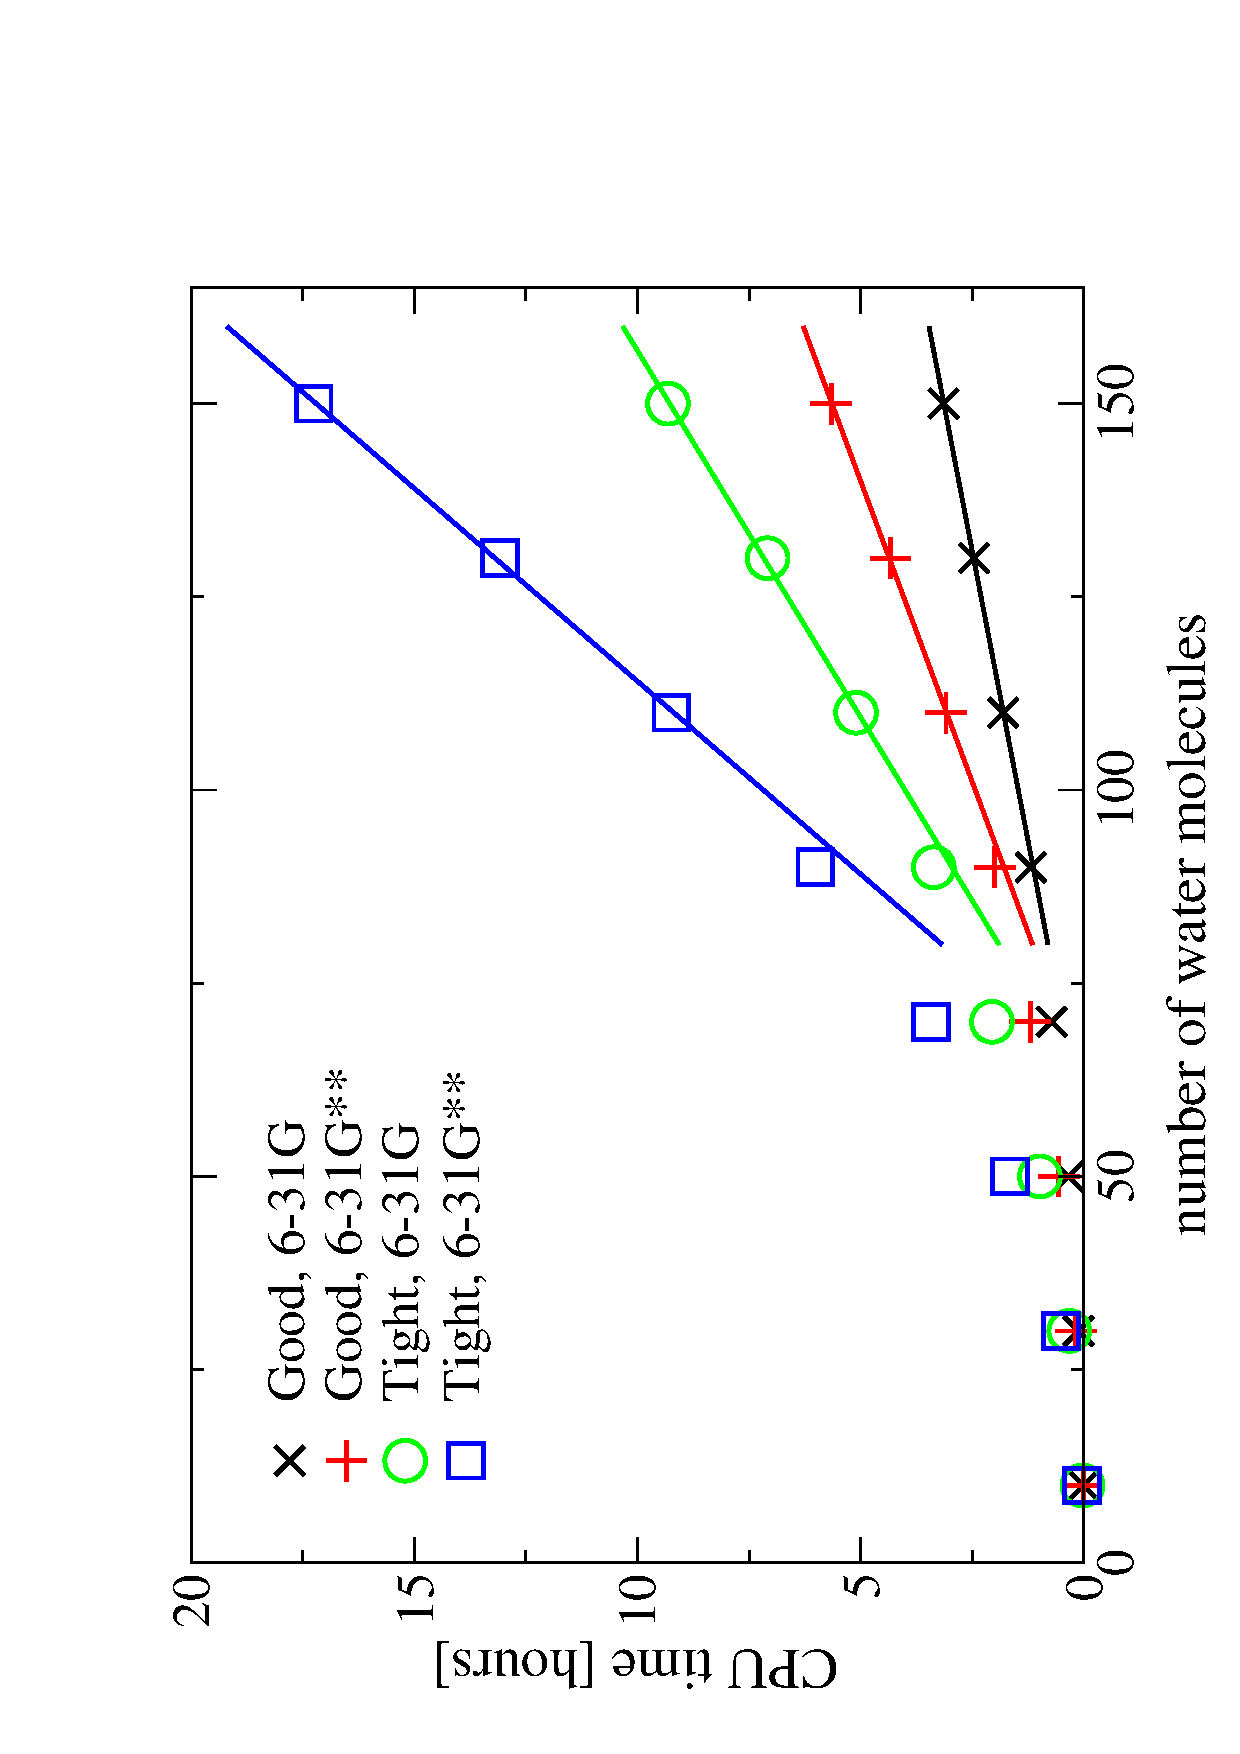
\includegraphics[angle=-90.00]{Gamma_h2o3D_6-31G_6-31Gss_G_T}}
\end{figure}

\begin{figure}[h]
  \caption{\protect
    QCTC CPU time of the fifth CPSCF iteration of third order for
    the water cluster sequence with the 6-31G and 6-31G** 
    basis sets and the {\tt GOOD} and {\tt TIGHT} 
    numerical thresholds (see text) controlling numerical
    precision of the result. The lines are fits to the 
    last three and four points, respectively.
  }\label{fig:Gamma_QCTC_Timing}
  \resizebox*{3.6in}{!}{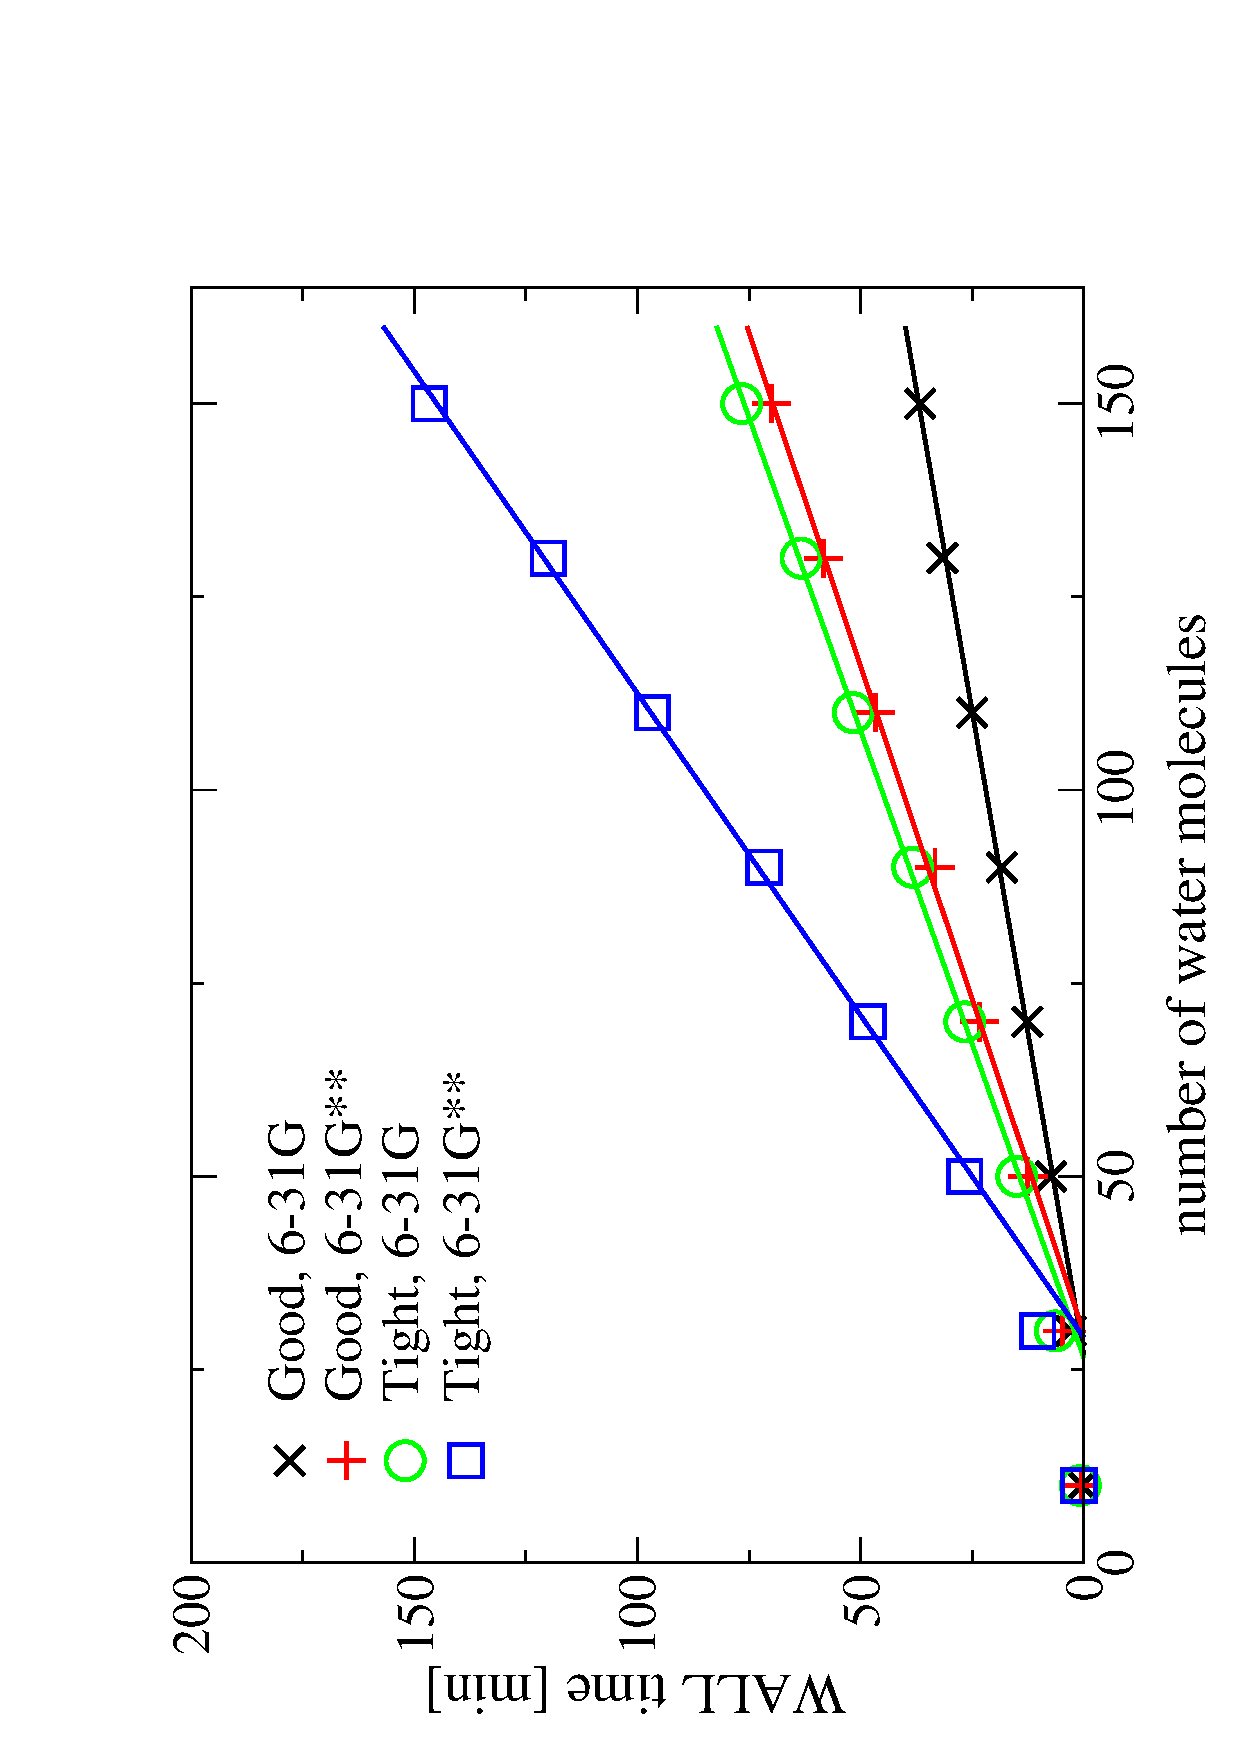
\includegraphics[angle=-90.00]{Gamma_QCTC_T}}
\end{figure}

\begin{figure}[h]
  \caption{\protect
    TC2 CPU time of the fifth CPSCF iteration of third order for
    the water cluster sequence with the 6-31G and 6-31G** 
    basis sets and the {\tt GOOD} and {\tt TIGHT} 
    numerical thresholds (see text) controlling numerical
    precision of the result. The lines are fits to the 
    last three and four points, respectively.
  }\label{fig:Gamma_TC2R_Timing}
  \resizebox*{3.6in}{!}{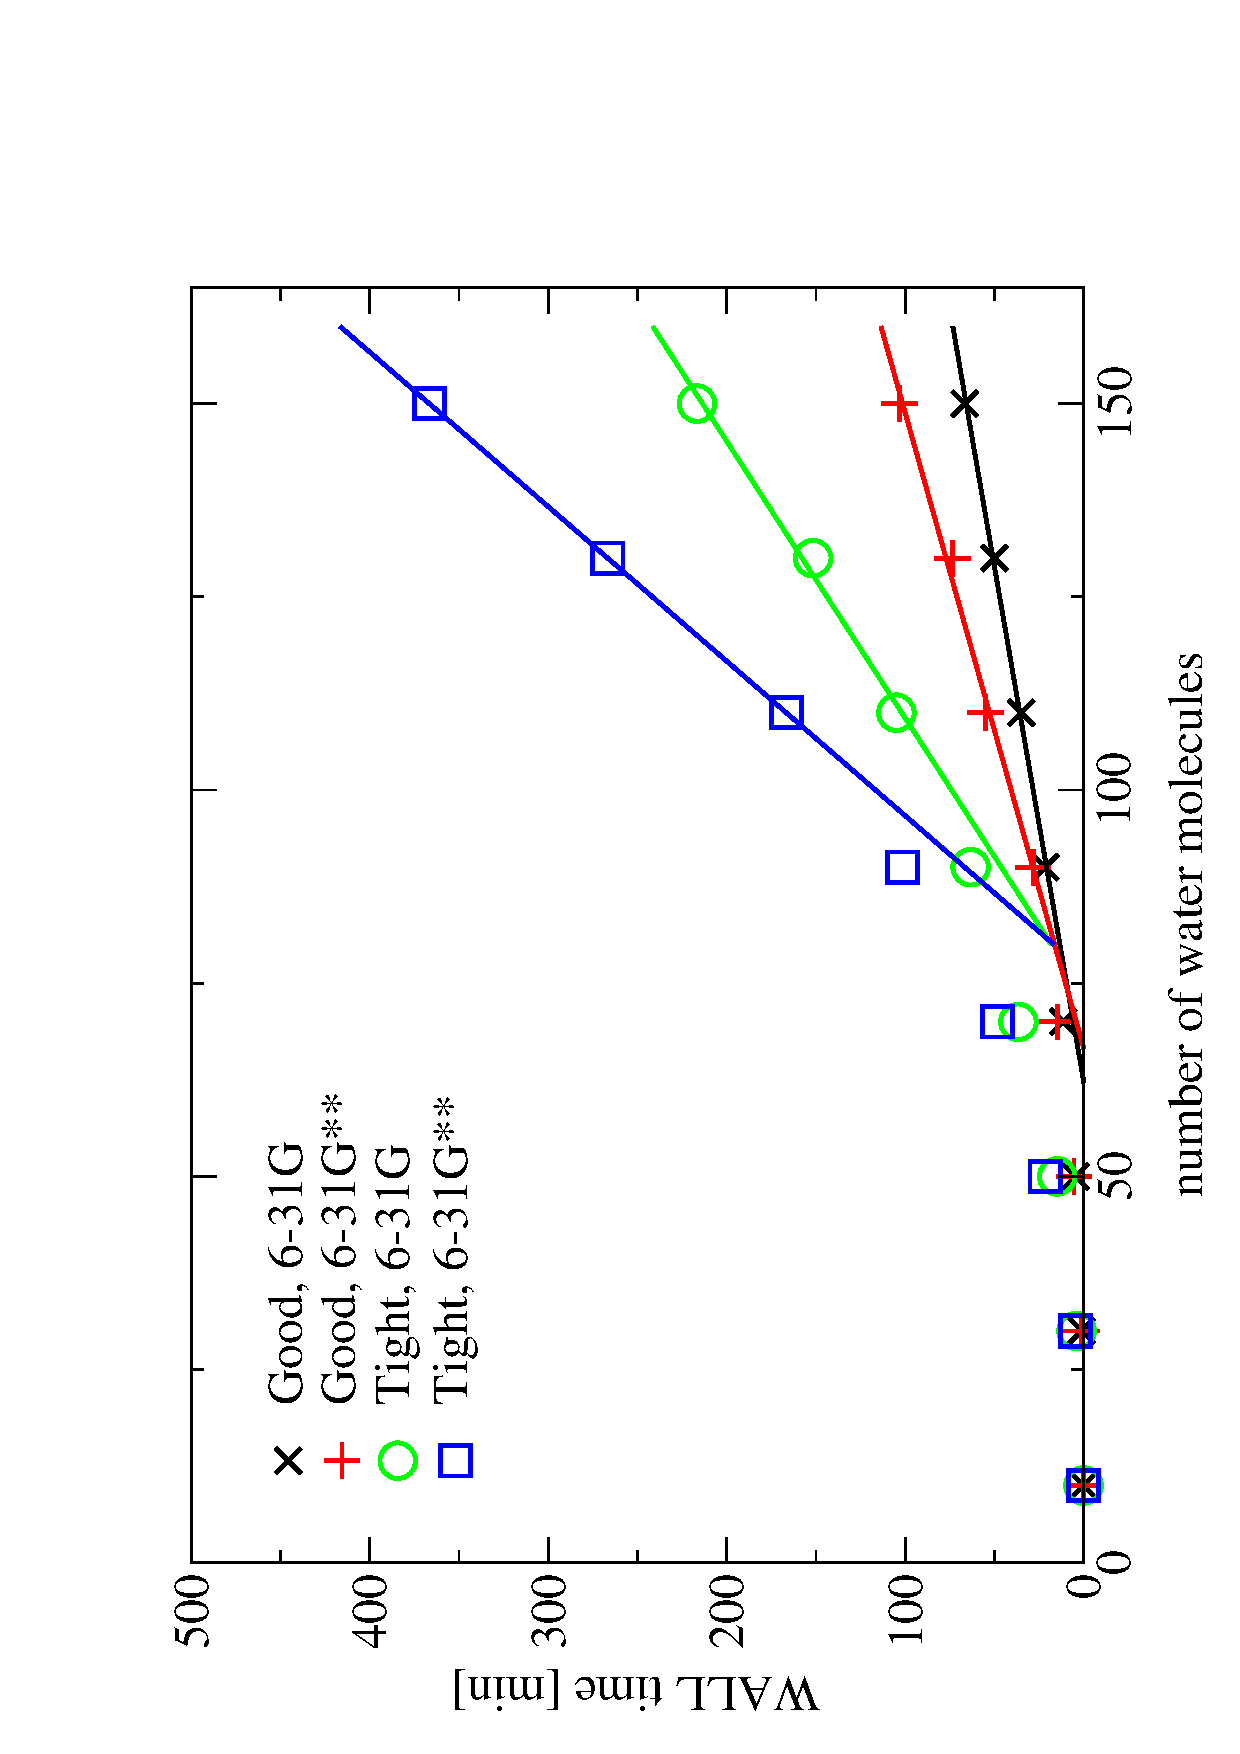
\includegraphics[angle=-90.00]{Gamma_TC2R_T}}
\end{figure}

\begin{figure}[h]
  \caption{\protect
    ONX CPU time of the fifth CPSCF iteration of third order for
    the water cluster sequence with the 6-31G and 6-31G** 
    basis sets and the {\tt GOOD} and {\tt TIGHT} 
    numerical thresholds (see text) controlling numerical
    precision of the result. The lines are fits to the 
    last three and four points, respectively.
  }\label{fig:Gamma_ONX_Timing}
  \resizebox*{3.6in}{!}{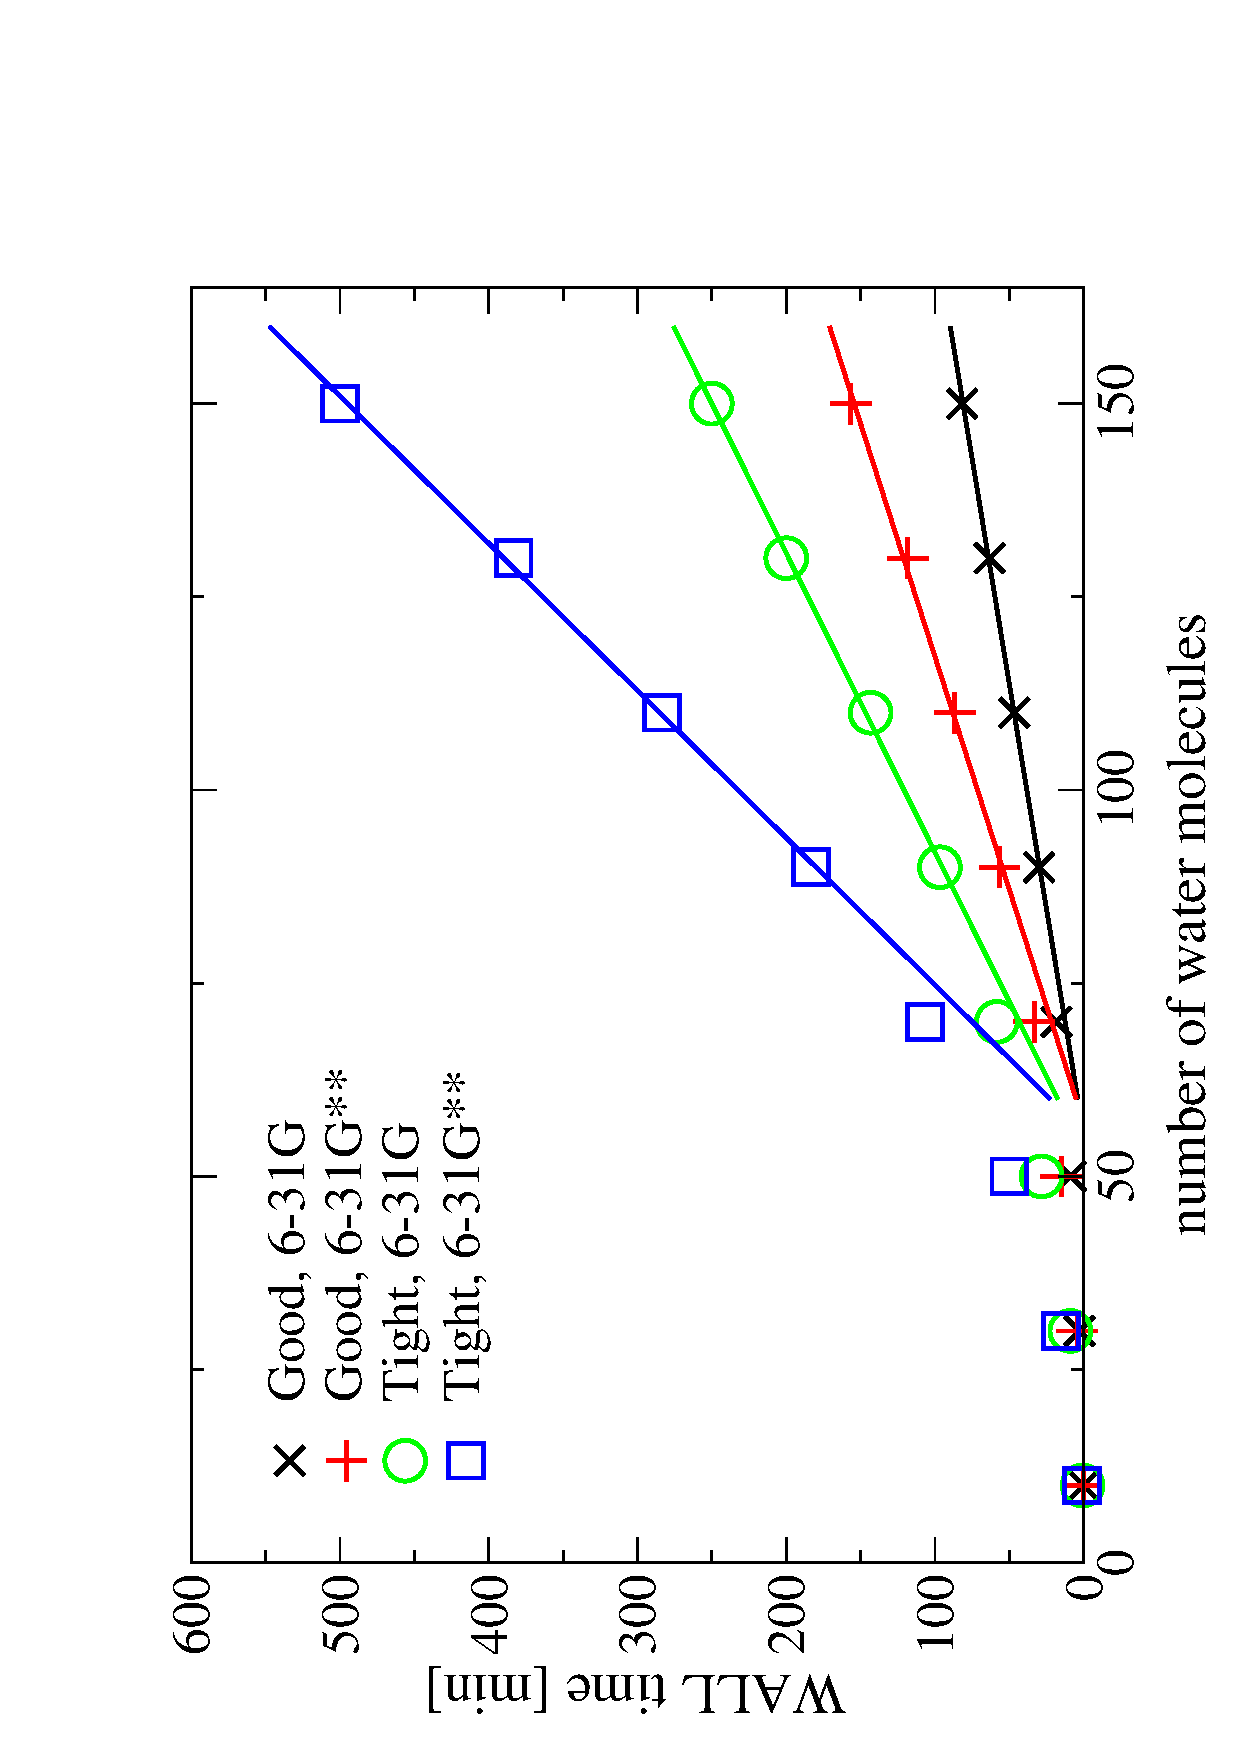
\includegraphics[angle=-90.00]{Gamma_ONX_T}}
\end{figure}


\begin{figure}[h]
  \caption{\bf [M: Maybe we should include this figure.  I kinda like it, 
      V: ok, if it makes the boss happy.]}
  \resizebox*{3.6in}{!}{\includegraphics[angle=-90.00]{Mix_h2o3D_6-31G_T.ps}}
\end{figure}

Linear scaling computation of the RHF/6-31G and RHF/6-31G** second hyperpolarizability,
achieved with Perturbed Projection, is shown for three-dimensional water clusters 
in Fig~\ref{fig:Gamma_scaling}.  These timings are the total CPU time for the fifth CPSCF cycle, 
including build time for $\F^{abc}$ ({\sc ONX} and {\sc QCTC}), 
iterative construction of $\D^{abc}$ (Perturbed Projection via {\sc TC2}) and all intermadiate
steps including the congruence tranformation.
A breakdown of the domminant contributions to these totals are given
in Figs~\ref{fig:Gamma_QCTC_Timing}-\ref{fig:Gamma_ONX_Timing}, which show timings for Coulomb 
summation ({\sc QCTC}), Perturbed Projection ({\sc TC2}), and excact exchange ({\sc ONX}).

\begin{figure}[t]
  \caption{\protect
    Superposition of the magnitudes of the RHF/6-31G density matrix
    derivative elements $D_{cd}$, $D^{x}_{cd}$, $D^{xx}_{cd}$ and $D^{xxx}_{cd}$
    along the $x$ axis with the separation of basis function centers
    for $\rm (H_2O)_{150}$. The density matrix 
    derivatives have been converged to within {\tt TIGHT} (e.g. 
    a matrix threshold $\tau=10^{-6}$ $[a.u.]$).
  }\label{fig:Superposition_Decay}
  \resizebox*{3.6in}{!}{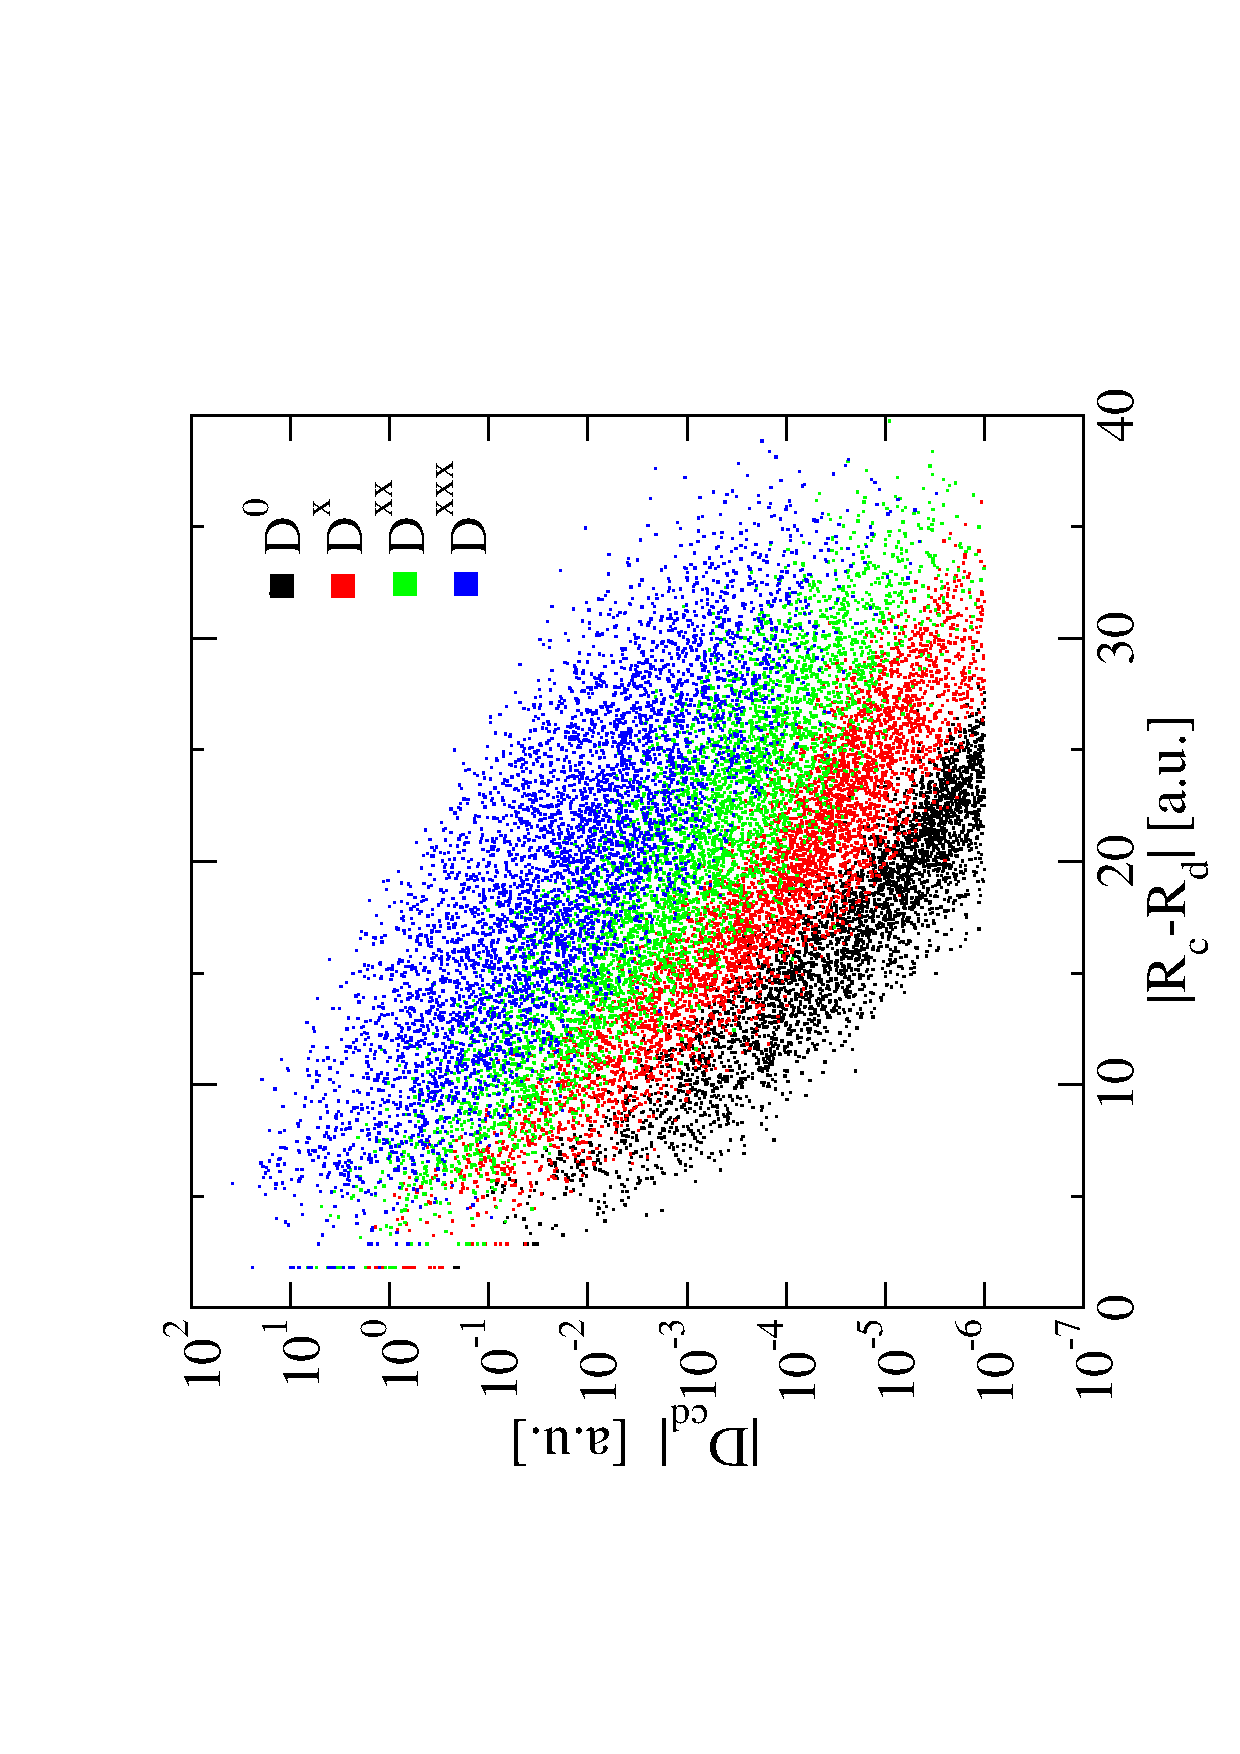
\includegraphics[angle=-90.00]{DMix_40pts}}
\end{figure}

Figure \ref{fig:Superposition_Decay} shows the magnitude of atom-atom blocks of density matrix derivatives
up to third order as a function of atom-atom distance when perturbed by a static electric field. 
The density response shows an approximate exponential decay as a function of internuclear distance, 
however the rate of decay slows with increasing order of the response.  We also note that, within
our convention of normalization, Eqs.~(\ref{}), the magnitude of the response functions are shifted
up with each order in the perturbation.

\newpage

\section{Discussion}

In our current formulation, the increase in magnitude and reduction of locality in elements of the 
response function makes achieving linear scaling more difficult with increasing order in perturbation. 
Nevertheless, linear scaling is achieved at the HF level of theory up to fourth order (i.e.~$\gamma_{abcd}$) 
in the total energy for three-dimensional systems and  non-trivial basis sets.  At fourth order,
Perturbed Projection and exact exchange were the dominant costs in solving the CPSCF equations,
as shown in Figs~\ref{}-\ref{}.  For the fourth order Perturbed Projection, $N$-scaling is achieved 
between 70 to 110 water molecules, depending on $\tau$.  Despite a nearly dense $D^{abc}$, the 
dominant work in its construction always involves multiplication with matrices that are significantly 
more sparse, as $\X^{abc}_i\X^{0}_i$ or $\X^{ab}_i\X^{c}_i$.   Likewise, $N$-scaling is achieved between 
70 to 90 water molecules for construction of the Hartree-Fock exchange contribution.  In this case, 
the approximate decay of the density matrix still leads to linear scaling through ordered skip out lists,
as described in Ref.~\onlinecite{ESchwegler97}.  In both cases, the increase in response function magnitude
is equivalent to tightening numerical thresholds, which increases the cost and delays the onset of linear
scaling. 

In principle, the evaluation of properties via expectation values, Eq.~(\ref{Np1Rule}), will involve
a different accumulation of errors relative to the $2n+1$ rule, Eqs.~(\ref{}-\ref{}). {\bf [M: It
would be great to have another coloumn for $\gamma$ at good computed at good so we can have this 
conversation.  Certainly, for N=5, the 2N+1 TIGHT results appear more accurate relative to VERYTIGHT.
How this plays out for GOOD and larger N is the question!]}.  

To investigate the numerical stability we compare the data calculated
with a {\tt TIGHT} numerical threshold ($10^{-6}$) with the polarizabilities
calculated using a {\tt GOOD} numerical threshold ($10^{-5}$). 
In tables \ref{tab:Alpha_1D_Values}-\ref{tab:Gamma_1D_Values} we find that
only 1-2 significant digit altered by reducing the threshold by two orders 
of magnitude. 

For example, a calculation of (H$_2$O)$_20$ with the {\tt VERYTIGHT} numerical threshold ($10^{-7}$) 
gives the following polarizabilities $\alpha_{zz}=7.142422\,a.u.$, $\beta_{zzz}=-12.033362\,a.u.$ and
$\gamma_{zzzz}=1411.425500\,a.u.$. We can conclude that the thresholds 
{\tt GOOD} and {\tt TIGHT} give approximatively 3-4 and 5-6 
correct digits respectivelly independently of the order of the response calculated.

The calculations of the first and second hyperpolarizabilities with the help of
the density matrix based $2n+1$ rule (See Tables \ref{tab:Beta_1D_Values} and \ref{tab:Gamma_1D_Values}) 
give about the same number of digit as the explicit calculations (i.e. 5-6 digits).
{\bf [M:I'm not sure this is right.  We need to see 2N+1 GOOD results.]}.

{\bf [M: We postpone further discussion about thresholding etc here untill we see what the GOOD 2N+1 results look like]}.

\newpage

\section{Conclusion}
We have extended the Perturbed Projection method for computation of 
the Coupled Pertrubed Self-Consistent-Field equations through higher order, 
and demonstrated linear scaling and error control through fourth order for 
three-dimensional systems and non-trivial basis sets.   In addition to 
achieving linear scaling,  Perturbed Projection for the computation of 
higher order response functions is quadratically convergent, simple to 
implement and numerically stable. 

We have shown that the density matrix response through fourth order is local 
upon a {\em global} electric perturbation, corresponding to an approximate 
exponential decay of matrix elements.  However, this locality decreases with
increasing order. {\bf [M: And here we postpone further discussion unitill
we have the GOOD results]}.
 A similar exponential decay
in the first order response corresponding to the {\em local} nuclear 
displacement has previously been demonstrated by Ochsenfeld and 
Head-Gordon \cite{Ochsenfeld97}. These key observations are expected to
hold generally for both local and global perturbations to insulating systems.  
We note also that the method is not unique to the TC2 generator or 
{\sc MondoSCF} $N$-scaling algorithms, but can be straightforwardly 
extended to other purification schemes such as TRS4 \cite{ANiklasson03} as
well as other electronic structure programs.

Convergence of the CPSCF equations for these systems (water cluster ...)
are typically achieved in about 10 cycles, independent of cluster size, basis set,
matrix threshold or order of the response calculated.

The perturbed projectro algorithm described in steps (\ref{FockBuild}-\ref{DDeriv}) and 
(\ref{PP1}-\ref{PP2})
can be easily extended to the linear scaling computation of
DFT and hybrid DFT models and a large class of static molecular properties
such as the geometrical derivatives so important
in the evaluation of the nuclear hessian, the nuclear magnetic
shielding tensor (NMR shift), indirect spin-spin coupling and
electronic g-tensor.

\begin{acknowledgments}
 This work has been supported by the US Department of Energy 
 under contract ???????????? and the ASCI project.  
 The Advanced Computing Laboratory of Los 
 Alamos National Laboratory is acknowledged.
 All the numerical computations have been
 performed on computing resources located at this facility.
\end{acknowledgments}


\bibliography{Response3}

\end{document}
